\documentclass[12pt,a4paper]{article}% 

%\usepackage{fontspec}
%\setmainfont{Times New Roman}
\usepackage{setspace}
\usepackage[a4paper,margin=1in]{geometry}
\usepackage{kbordermatrix}
\usepackage{amsmath}
\usepackage{longtable}
\usepackage{pgfplots}
\usepackage{ragged2e}
\usepackage{biblatex}
\usepackage[noend]{algorithmic}
\usepackage{listings}
\usepackage{fancyhdr}
\usepackage{booktabs}
	\lstset{
		frame=tb, % draw a frame at the top and bottom of the code block
		tabsize=4, % tab space width
		showstringspaces=false, % don't mark spaces in strings
		numbers=left, % display line numbers on the left
		commentstyle=\color{green}, % comment color
		keywordstyle=\color{blue}, % keyword color
		stringstyle=\color{red} % string color
	}

\usepackage [english]{babel}
\usepackage [autostyle, english = american]{csquotes}
\MakeOuterQuote{"}
\usepackage{pgfplots,amsmath}
\pgfplotsset{compat=1.12}

\pagestyle{fancy}
\fancyhf{}% Clear header/footer
\fancyfoot[C]{\thepage}% \fancyfoot[R]{\thepage}
\renewcommand{\headrulewidth}{0 pt}% Default \headrulewidth is 0.4pt
\renewcommand{\footrulewidth}{0.4pt}% Default \footrulewidth is 0pt


\renewcommand{\footrulewidth}{0.4pt}

\newcommand{\TITLE}[1]{\item[#1]}
\renewcommand{\algorithmiccomment}[1]{$/\!/$ \parbox[t]{4.5cm}{\raggedright #1}}
\newbox\fixbox
\renewcommand{\algorithmicdo}{\setbox\fixbox\hbox{\ {} }\hskip-\wd\fixbox}
\newcommand{\algcost}[2]{\strut\hfill\makebox[1.5cm][l]{#1}\makebox[4cm][l]{#2}}
\usetikzlibrary{arrows,automata,positioning}
\usetikzlibrary{arrows.meta}
\usetikzlibrary{calc}

\pgfmathsetseed{3}
\newcommand*{\Comb}[2]{{}^{#1}C_{#2}}



\begin{document}
	
	\begin{titlepage}
		\topmargin = -100pt
		\footskip = 10pt
		\title{	
		\setstretch{1.2}
		\textbf{\large Title: FACE RECOGNITION BASED AUTOMATIC ATTENDANCE MANAGEMENT SYSTEM USING DEEP LEARNING}\\ \bigskip \bigskip
		\textbf{\large A Report Submitted in Partial Fulfillment of the Requirements\\
			for the\\
			6th Semester B.Tech. Summer Internship\\
			(Mode of Internship is ONLINE) \\ \bigskip By \\ \bigskip
			Saranga Pani Nath 1815009\\
			Nilam Kumar Kalita	1815127 \\ 		\bigskip
			Under the Guidance of \\ 
			Dr. Malaya Dutta Borah \\
			Assistant Professor\\ \bigskip	
		}
		
\includegraphics[width=0.38 \textwidth]{./NIT_Silchar_logo.png} \\		
		\textbf{{\large Computer Science and Engineering Department}}\\
		\textbf{\large NATIONAL INSTITUTE OF TECHNOLOGY, SILCHAR\\ \bigskip ASSAM}\\		
		\textbf{\date{May-June 2021}	}
		}
		\clearpage\maketitle
		\thispagestyle{empty}
	\end{titlepage}

	\tableofcontents
	\pagebreak
	\section{Abstract }
	\justify
	Lorem ipsum
		
	\pagebreak
   \section{Introduction }
   \paragraph{}
   \justify
	Lorem ipsum
        \pagebreak
        
        
    \section{Literature Survey}
	\begin{longtable}{|p{2cm}|p{4cm}|p{7cm}|}
	
	 
	\hline
	%%%%%%%%%%%%%%%%%%%%%%%%%%%%%%%%%%%%%%%%%%%%%%%%%%%%%%%%
	\textbf{Sl No.} & \textbf{Research Paper} & \textbf{Approaches}\\
	\hline
	1. & Face Recognition Based 
	Attendance Management System 
	\textit{\textbf{ - Smitha, Pavithra S Hegde, Afshin}}
	& \textbf{a.} Firstly we will create a dataset by capturing the images of the students. 
	The region of interest(ROI)  will be extracted from the images. 
	The cropped images will be resized  to a particular pixel position. 
	The images will be converted from RGB to gray scale images.
	\\
	\hline
	&  & \textbf{b.} By using Haar-Cascade classifier, the face detection is performed. The features of the images will be extracted.
	A rectangle around the face will be created , having three parameters:
	\begin{itemize}
		\item \textbf{scaleFactor:} scaleFactor is used to indicate how much an image must be reduced in each image scale.
		\item \textbf{minNeighbors:}   minNeighbors specifies how many neighbors each candidate rectangle must have.
		\item \textbf{minSize:}  minSize specifies the minimum object size.
	\end{itemize}\\
	\hline
	&  & \textbf{c.} Face recognition process can be divided into various steps:
	\begin{itemize}
		\item Prepare training data.
		\item Train face recognizer.
		\item Prediction.
		\item Local Binary Pattern Histogram(LBP) is used as a face           recogniser.
		\item LBPs are converted into decimal numbers.
		\item The decimal values are plotted in histograms.
		\item For each images of the in the training data histograms          will be formed.
		\item Finally Histogram of the face to be recognised is              calculated and compared with the already computed              histograms and returns the best matched label associated       with the student it belongs to.
	\end{itemize}\\
	\hline
	& & \textbf{d.} After recognition the recognized faces will be marked as present in the excel sheet and the rest will be marked as absent and the list of absentees will be mailed to the respective faculties.\\ 
	\hline 
	%%%%%%%%%%%%%%%%%%%%%%%%%%%%%%%%%%%%%%%%%%%%%%%%%%%%%%%%
	
	2. & Using Siamese Networks with Transfer Learning for Face Recognition on Small-Samples Datasets \textit{\textbf{ - Mohsen Heidari,Kazim Fouladi-Ghaleh}}
	& \textbf{a.} The authors of this paper used transfer learning to solve the face recognition problem with small dataset. For this, they used pre trained VGG-16 as the convolutional neural network in Siamese network for feature extraction and fine tune it.  
	\\
	\hline		
	&  & \textbf{b.} They removed all fully connected layers from VGG-16 and inserted three fully connected layers with RELU functions. Then during training they freezed all the convolution layers except the last one. The network input size was 128*128*3.
	\\ 
	\hline
	&  & \textbf{c.} To train the proposed network they used contrastive loss function. It tries to minimize the square Euclidean distance for similar pairs of images and maximize this distance for dissimilar pair of images, so that similar samples will get closer and dissimilar will get farer. 
	\\ 
	\hline
	&  & \textbf{d.} The authors used LFW dataset in this approach. This date set has almost 13000 facial images (about 1680 persons) with labelled with person name. Each image is a color image with size of 250*250. In this research, the authors got $ 95.62 \% $ accuracy.
	\\ 
	\hline
	%%%%%%%%%%%%%%%%%%%%%%%%%%%%%%%%%%%%%%%%%%%%%%%%%%%%%%%%%%%%%%%
	3. & Face Recognition based on Convolution Siamese
	Networks \textit{\textbf{ - Haoran Wu, Zhiyong Xu, Jianlin Zhang, Wei Yan, Xiao Ma}}
	& \textbf{a.} In this paper also, the authors used Siamese network for face recognition. The authors proposed a new CNN architecture for feature extraction. In the designed system, they divided the recognition task into two part – face detection and then recognition. Face detection is based on cascade classification and they adopt Haar features to improve the accuracy step by step.  
	\\
	\hline		
	&  & \textbf{b.} The architecture mainly consists of two pairs of convolution and pooling layers followed by three convolution layers. The details about dimensions of each layer is given in the paper. 
	\\ 
	\hline
	&  & \textbf{c.} During training, they adopt layer by layer training method. Gradient feedback principal and SGD are used for the training of the Siamese network. They used their own dataset and for each person they took 30 images with different alignments and face expressions so that the accuracy of the model is increased. In this research, the authors got $ 98.21\% $ accuracy.
	\\ 
	\hline		
	%%%%%%%%%%%%%%%%%%%%%%%%%%%%%%%%%%%%%%%%%%%%%%%%%%%%%%%%
	\caption{\texttt{FACE RECOGNITION BASED AUTOMATIC ATTENDANCE MANAGEMENT SYSTEM USING DEEP LEARNING\\}} % needs to go inside longtable environment
	\label{tab:myfirstlongtable}
\end{longtable}
%\end{table} 

Table \ref{tab:myfirstlongtable} shows the list of similar works.
    
    
        
       
    \section{The Concept of Block Chain }
    \subsection{Block chain overview}
    \paragraph{}
    \justify
    Lorem ipsum
    
    The key characteristics of block chain are:
    \begin{enumerate}
    	\item Distributed : Blo
    \end{enumerate}
    
    \subsection{new subsec}
    \paragraph{}
    \justify
    Lorem ipsum
    
    
    \subsection{new subsec}
    \paragraph{}
    \justify
    Lorem ipsum. \\
    
    Now the following points can be seen from the above discussion:
    
    \begin{enumerate}
    	\item The proces
    	
    \end{enumerate}

	\pagebreak
		
	\section{new sec }
	\paragraph{}
	\justify
Lorem ipsum
	\begin{enumerate}
		\item RQ1 : Fair
	\end{enumerate}
	\pagebreak
	
	\section{new sec}
	\begin{flushleft}
		\justify
		In the following
		\subsection{new subsec}
		\begin{flushleft}
			\justify
			The central question we address here is that \textit{Does thng?}\\\\
			It becomes imperati 
			
		\end{flushleft}
	
		\subsection{new subsec}
		\begin{flushleft}
			\justify
			The question that we address here is - \textit{Doe ?}\\\\
			This is a central and
			\begin{center}
			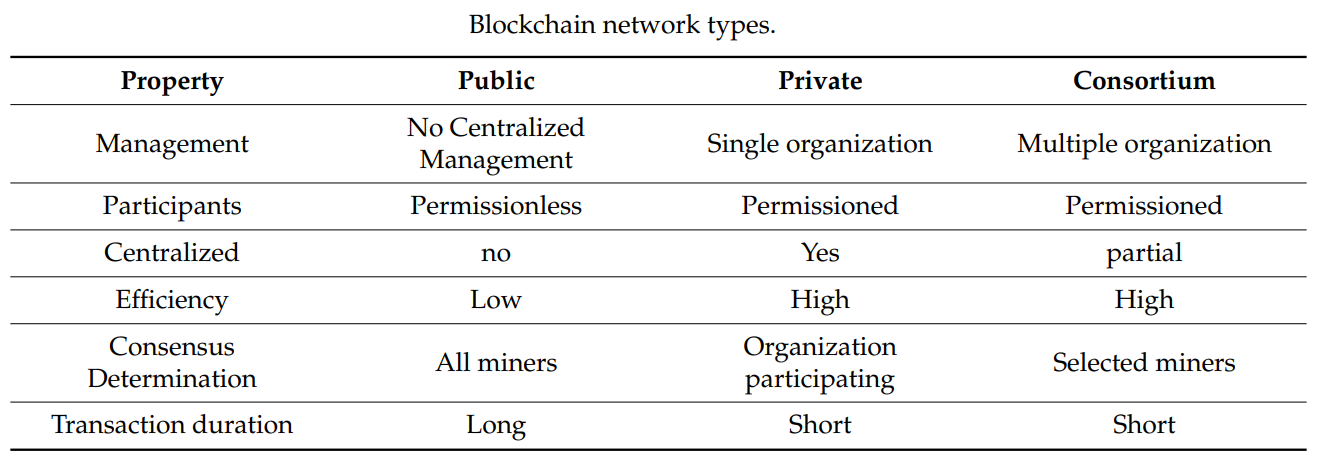
\includegraphics[width=0.90 \textwidth]{./blockchain_network_types.png}
			\\\textbf{Figure 1}: Comparison of different blockchain network types.
			\end{center}
		\end{flushleft}
	
		\subsection{RQ3: Uniqueness}
		\begin{flushleft}
			\justify
			 Another critical question that we need to address is Uniqueness/Un-Reusability - \textit{Is the means ?}\\\\
			First up
			\begin{center}
				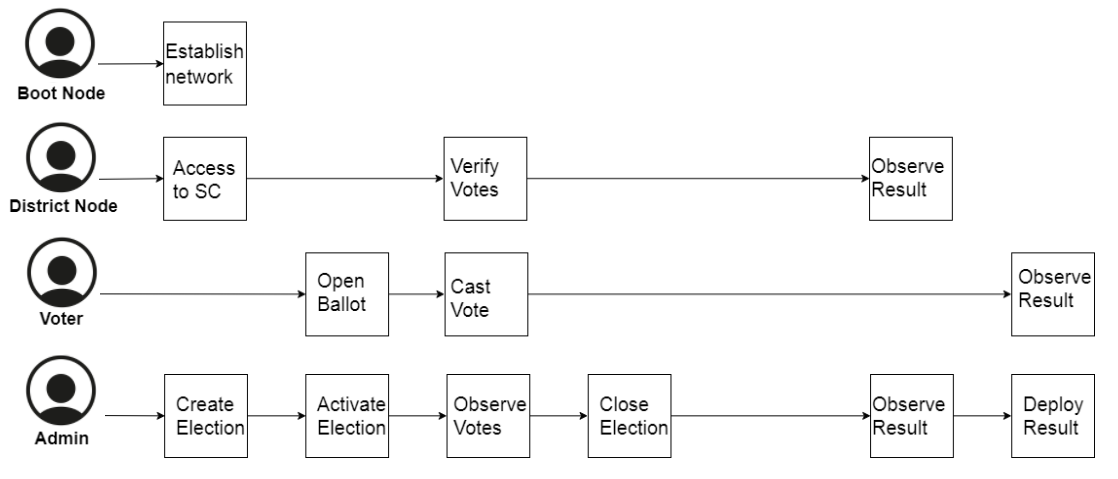
\includegraphics[width=0.90 \textwidth]{./flow_diagram_CA.png}	
				\\\textbf{Figure 2}: Probable functionalities of various nodes that can be incorporated in our e-voting system.
			\end{center}
				
		\end{flushleft}
	
	
		\subsection{new subsec}
		\begin{flushleft}
			\justify
			\textit{Is there anys?}\\
			
			Maintaining integr
			
			
		\end{flushleft}
		
		\subsection{new subsec}
		\begin{flushleft}
			\justify
			\textit{Is the system ders?}\\
			
			The Prêt à Vo
			
			
		\end{flushleft}
		\subsection{new subsec}
		\begin{flushleft}
			\justify
			 \textit{Does the syst?}\\ \\
			The anomaly 
			
		\end{flushleft}
		\subsection{new subsec}
		\begin{flushleft}
			\justify
			\textit{Does g the results ?}\\
			
			With a central aut 
			
			
		\end{flushleft}
		
		\subsection{new subsec}
		\begin{flushleft}
			\justify
			\textit{Is thection ?}\\
			
			The adjudication  
			
		\end{flushleft}
		
		\subsection{new subsec }
		\begin{flushleft}
			\justify
			\textit{What solution does ult to use?}\\
			
			Old age and illiterat\\
			
		\end{flushleft}
	
	
	\end{flushleft}

	\pagebreak
	\section{Discussion}
	\justify
		The study indicates that iability,etc.\\ \\
		
	\pagebreak
	\section{Conclusion}
	\justify
		This paper aims to do a systematic review of the recent literatures on blockchain based e-voting system. Its starts with information on current 

	\pagebreak
	
	
	\begin{thebibliography}{9}
		\bibitem{ref1}  khbkbk

		
		\bibitem{ref2}

		
		\bibitem{ref3}

		
		
		\bibitem{ref4}

		
		\bibitem{ref5}

		
		\bibitem{ref6}

		
		\bibitem{ref7}

		
		\bibitem{ref8}

		
		
		\bibitem{ref9}

		
		\bibitem{ref10}

		
		\bibitem{ref11}

		
		
		\bibitem{ref12}

		
		
		\bibitem{ref13}

		 
	\end{thebibliography}
	
	
\end{document} 
